% Options for packages loaded elsewhere
\PassOptionsToPackage{unicode}{hyperref}
\PassOptionsToPackage{hyphens}{url}
%
\documentclass[
]{article}
\usepackage{amsmath,amssymb}
\usepackage{iftex}
\ifPDFTeX
  \usepackage[T1]{fontenc}
  \usepackage[utf8]{inputenc}
  \usepackage{textcomp} % provide euro and other symbols
\else % if luatex or xetex
  \usepackage{unicode-math} % this also loads fontspec
  \defaultfontfeatures{Scale=MatchLowercase}
  \defaultfontfeatures[\rmfamily]{Ligatures=TeX,Scale=1}
\fi
\usepackage{lmodern}
\ifPDFTeX\else
  % xetex/luatex font selection
\fi
% Use upquote if available, for straight quotes in verbatim environments
\IfFileExists{upquote.sty}{\usepackage{upquote}}{}
\IfFileExists{microtype.sty}{% use microtype if available
  \usepackage[]{microtype}
  \UseMicrotypeSet[protrusion]{basicmath} % disable protrusion for tt fonts
}{}
\makeatletter
\@ifundefined{KOMAClassName}{% if non-KOMA class
  \IfFileExists{parskip.sty}{%
    \usepackage{parskip}
  }{% else
    \setlength{\parindent}{0pt}
    \setlength{\parskip}{6pt plus 2pt minus 1pt}}
}{% if KOMA class
  \KOMAoptions{parskip=half}}
\makeatother
\usepackage{xcolor}
\usepackage[margin=1in]{geometry}
\usepackage{longtable,booktabs,array}
\usepackage{calc} % for calculating minipage widths
% Correct order of tables after \paragraph or \subparagraph
\usepackage{etoolbox}
\makeatletter
\patchcmd\longtable{\par}{\if@noskipsec\mbox{}\fi\par}{}{}
\makeatother
% Allow footnotes in longtable head/foot
\IfFileExists{footnotehyper.sty}{\usepackage{footnotehyper}}{\usepackage{footnote}}
\makesavenoteenv{longtable}
\usepackage{graphicx}
\makeatletter
\def\maxwidth{\ifdim\Gin@nat@width>\linewidth\linewidth\else\Gin@nat@width\fi}
\def\maxheight{\ifdim\Gin@nat@height>\textheight\textheight\else\Gin@nat@height\fi}
\makeatother
% Scale images if necessary, so that they will not overflow the page
% margins by default, and it is still possible to overwrite the defaults
% using explicit options in \includegraphics[width, height, ...]{}
\setkeys{Gin}{width=\maxwidth,height=\maxheight,keepaspectratio}
% Set default figure placement to htbp
\makeatletter
\def\fps@figure{htbp}
\makeatother
\setlength{\emergencystretch}{3em} % prevent overfull lines
\providecommand{\tightlist}{%
  \setlength{\itemsep}{0pt}\setlength{\parskip}{0pt}}
\setcounter{secnumdepth}{-\maxdimen} % remove section numbering
\usepackage{amsmath,epsfig}
\usepackage{amssymb,amsthm}
\usepackage[all]{xy}
\usepackage{xcolor}
\usepackage{mathtools}
\usepackage{mathrsfs}
% Needed to have supplementary figures labled as 'S1', 'S2', etc.
\newcommand{\beginsupplement}{
  \setcounter{table}{0}  
  \renewcommand{\thetable}{S\arabic{table}} 
  \setcounter{figure}{0} 
  \renewcommand{\thefigure}{S\arabic{figure}}
}
\newtheorem{lemma}{Lemma}
\newtheorem{theorem}{Theorem}

\usepackage{tabularx}
\usepackage{makecell}
\usepackage{multirow}

% uncomment the following lines for line numbers
%\usepackage[left]{lineno}
%\linenumbers
\usepackage{float}
\ifLuaTeX
  \usepackage{selnolig}  % disable illegal ligatures
\fi
\usepackage{bookmark}
\IfFileExists{xurl.sty}{\usepackage{xurl}}{} % add URL line breaks if available
\urlstyle{same}
\hypersetup{
  pdftitle={Multiple blood-feeding modeling study},
  pdfauthor={Kyle J.-M. Dahlin, Michael Robert, Lauren Childs},
  hidelinks,
  pdfcreator={LaTeX via pandoc}}

\title{Multiple blood-feeding modeling study}
\author{Kyle J.-M. Dahlin, Michael Robert, Lauren Childs}
\date{May 14, 2024}

\begin{document}
\maketitle

\section{Introduction}\label{introduction}

Mosquito-borne diseases are a big problem.

Multiple blood-feeding, in its many forms, is a phenomenon that may
multiply the transmission of mosquito-borne parasites.

\subsection{Mechanisms and processes of mosquito
blood-feeding}\label{mechanisms-and-processes-of-mosquito-blood-feeding}

Descriptions and diagrams

\begin{figure}[H]
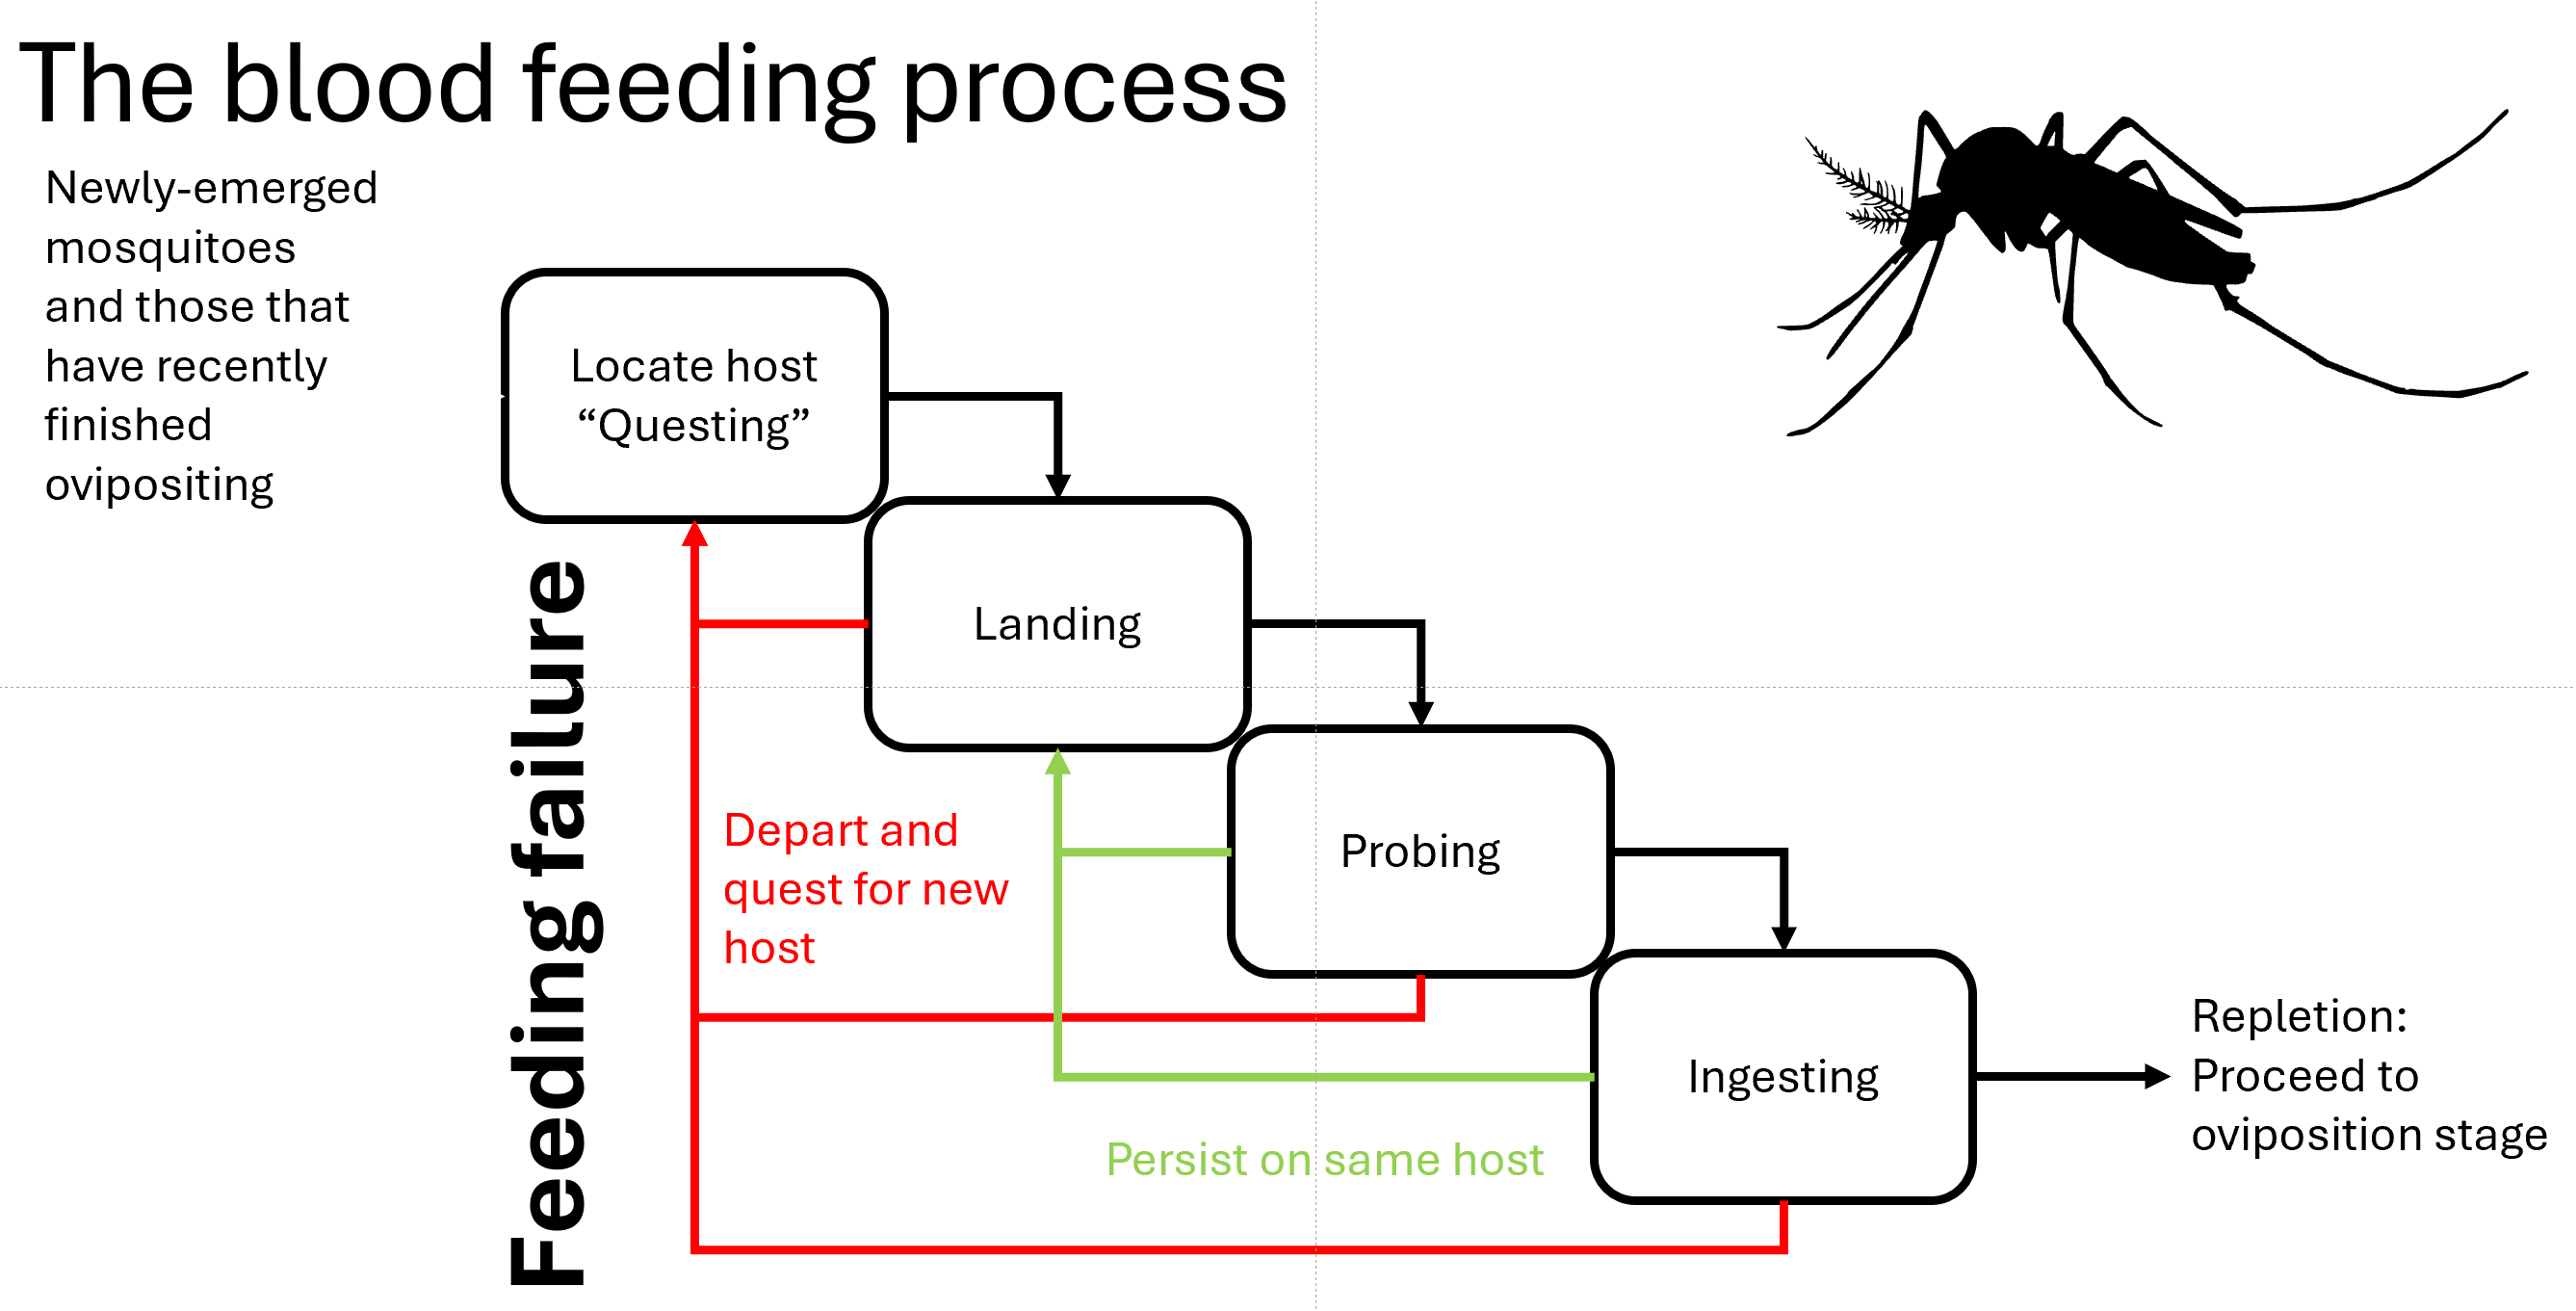
\includegraphics[width=400px,]{./figures/process_cartoon_draft} \caption{Cartoon of the mosquito blood-feeding process.}\label{fig:figure-1}
\end{figure}

\section{Methods}\label{methods}

\subsection{Box: Modeling processes with phase-type
distributions}\label{box-modeling-processes-with-phase-type-distributions}

\subsection{Model formulation}\label{model-formulation}

\subsection{Parameterization}\label{parameterization}

We assume the following parameter values for the biting parameters

\begin{longtable}[]{@{}
  >{\raggedright\arraybackslash}p{(\columnwidth - 4\tabcolsep) * \real{0.1412}}
  >{\raggedright\arraybackslash}p{(\columnwidth - 4\tabcolsep) * \real{0.7882}}
  >{\raggedleft\arraybackslash}p{(\columnwidth - 4\tabcolsep) * \real{0.0706}}@{}}
\toprule\noalign{}
\begin{minipage}[b]{\linewidth}\raggedright
Symbol
\end{minipage} & \begin{minipage}[b]{\linewidth}\raggedright
Description
\end{minipage} & \begin{minipage}[b]{\linewidth}\raggedleft
Value
\end{minipage} \\
\midrule\noalign{}
\endhead
\bottomrule\noalign{}
\endlastfoot
\(p_L\) & Probability of progressing from landing to probing & 0.70 \\
\(\lambda_L\) & Exit rate from landing stage (per minute) & 0.10 \\
\(p_P\) & Probability of progressing from probing to ingesting & 0.80 \\
\(\lambda_P\) & Exit rate from probing stage (per minute) & 0.20 \\
\(p_G\) & Probability of progressing from ingesting to ovipositing &
0.90 \\
\(\lambda_G\) & Exit rate from ingestion stage (per minute) & 1.00 \\
\(f\) & Probability of seeking a new vertebrate host given feeding
failure & 0.66 \\
\end{longtable}

and the following for the remaining model parameters

\begin{longtable}[]{@{}llr@{}}
\toprule\noalign{}
Symbol & Description & Value \\
\midrule\noalign{}
\endhead
\bottomrule\noalign{}
\endlastfoot
\(\eta\) & Extrinsic incubation rate & 0e+00 \\
\(\mu\) & Mosquito mortality rate & 0e+00 \\
\(\gamma\) & Return to blood-feeding rate & 0e+00 \\
\(\gamma_H\) & Host recovery rate & 0e+00 \\
\(\mu_H\) & Host mortality rate & 0e+00 \\
\(K_H\) & Host carrying capacity & 1e+07 \\
\(K_L\) & Larval mosquito carrying capacity & 3e+02 \\
\(\rho_L\) & Larval mosquito maturation rate & 0e+00 \\
\(\mu_L\) & Larval mosquito mortality rate & 0e+00 \\
\(\varphi\) & Eggs per female per day & 0e+00 \\
\(\beta_P\) & Probing transmission probability & 1e+00 \\
\(\beta_G\) & Ingestion transmission probability & 1e+00 \\
\(\beta_H\) & To-host transmission probability & 1e+00 \\
\(\beta_V\) & To-mosquito transmission probability & 1e+00 \\
\(\lambda_Q\) & Questing rate & 0e+00 \\
\end{longtable}

\subsection{Simulation}\label{simulation}

We simulate a set of measurements of the time it takes for a single
mosquito seeking a blood meal on a specific host to no longer seek a
blood meal. This data is heavily censored: we don't have information on
whether the mosquito successfully completed a blood meal or if it was
disrupted at any point in the feeding process. This simulation does not
take into account the time that the mosquito spends questing, that is,
we assume it has already located a suitable host to feed upon.

These parameters lead to a phase-type distributed waiting time for
blood-feeding parameterized by the sub-intensity matrix \(A\) given by
\[
A = \begin{bmatrix}-\lambda_{L}+\left(1-f\right)\left(1-p_{L}\right)\lambda_{L} & p_{L}\lambda_{L} & 0\\
\left(1-f\right)\left(1-p_{P}\right)\lambda_{P} & -\lambda_{P} & p_{p}\lambda_{P}\\
\left(1-f\right)\left(1-p_{G}\right)\lambda_{G} & 0 & -\lambda_{G}
\end{bmatrix}  = \begin{bmatrix} -0.0898 & 0.07 & 0\\
0.0136 & -0.2 & 0.16\\
0.034 & 0 & -1
\end{bmatrix}
\] and initial vector \(\alpha = \left(1,0,0\right)\).

This distribution takes the following approximate shape and has a mean
of 16.8353168 minutes and standard deviation of 13.5063023 minutes. The
5\% and 95\% quantiles are at 2.0691565 minutes and 42.9387666 minutes,
respectively.

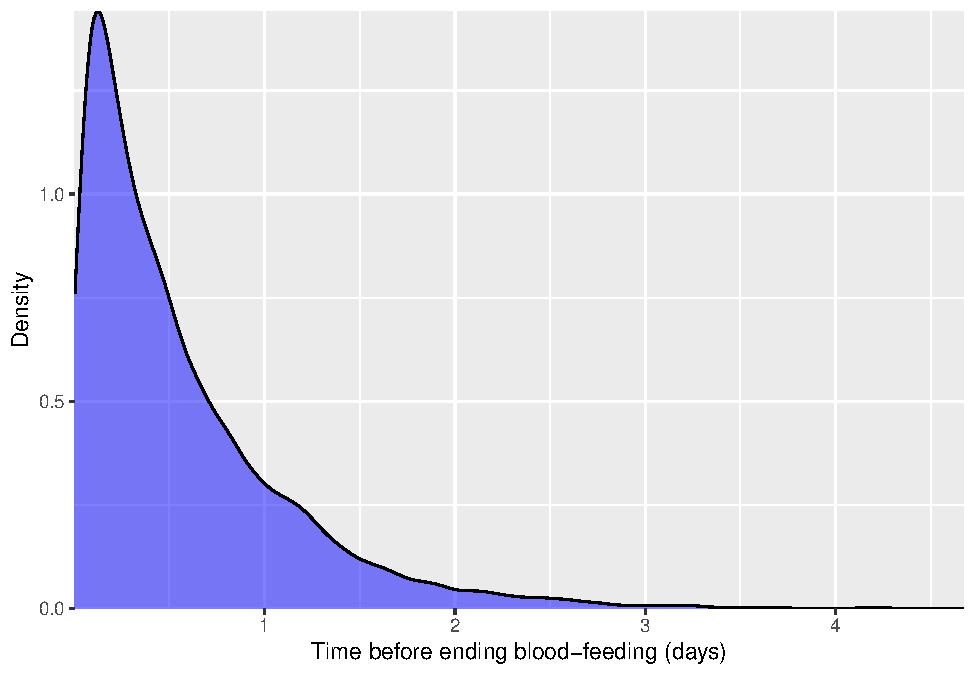
\includegraphics{F:/GitHub/MBF_models/doc/study_files/figure-latex/plot-simulation-1}
We will use this simulated data set as a proxy for real data that might
be collected to study the effects of multiple blood-feeding on
transmission.

\section{Results: Equilibrium
analysis}\label{results-equilibrium-analysis}

\subsection{Basic reproduction number}\label{basic-reproduction-number}

\subsection{Existence and stability of
equilibria}\label{existence-and-stability-of-equilibria}

\section{Results: Sensitivity
analysis}\label{results-sensitivity-analysis}

\subsection{Relationships among reproduction numbers and blood-feeding
parameters}\label{relationships-among-reproduction-numbers-and-blood-feeding-parameters}

\begin{figure}[H]
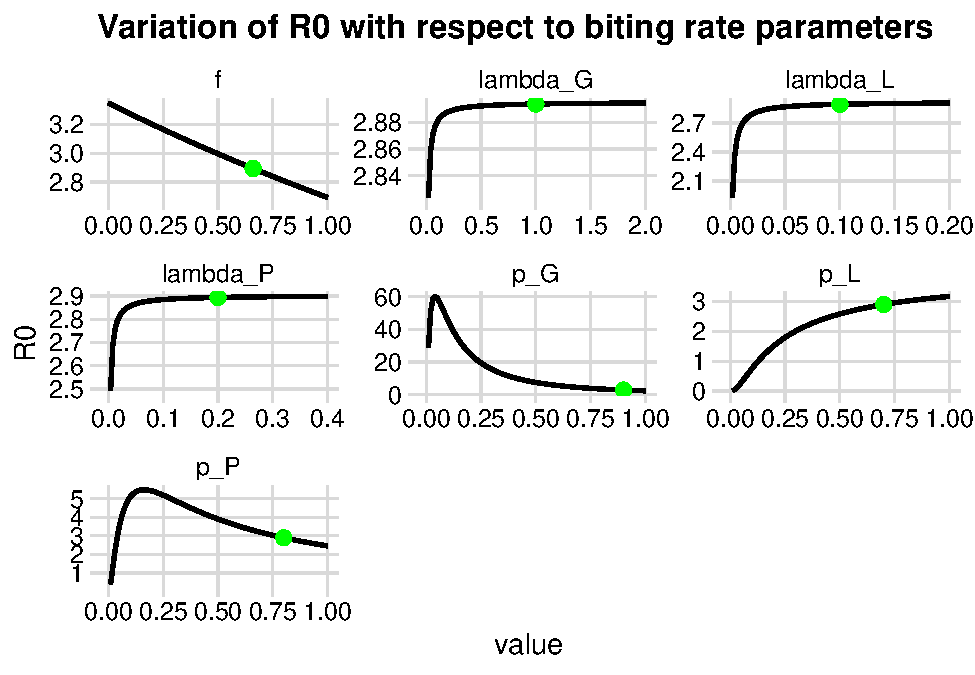
\includegraphics{F:/GitHub/MBF_models/doc/study_files/figure-latex/R0-monotonicity-plots-1} \caption{The basic reproduction and reproductive numbers as functions of the biting rate parameters. In each figure, only the labeled parameter is being varied. All other parameters are as in Tables 1 and 2.}\label{fig:R0-monotonicity-plots-1}
\end{figure}
\begin{figure}[H]
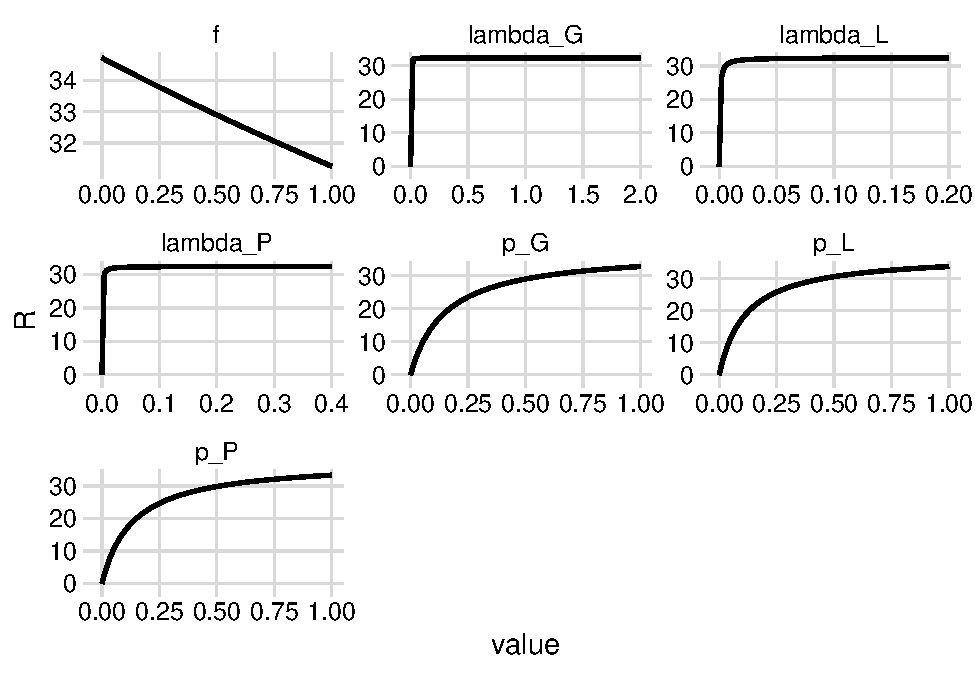
\includegraphics{F:/GitHub/MBF_models/doc/study_files/figure-latex/R0-monotonicity-plots-2} \caption{The basic reproduction and reproductive numbers as functions of the biting rate parameters. In each figure, only the labeled parameter is being varied. All other parameters are as in Tables 1 and 2.}\label{fig:R0-monotonicity-plots-2}
\end{figure}

\subsection{PRCCs of R0 or R and blood-feeding
parameters}\label{prccs-of-r0-or-r-and-blood-feeding-parameters}

Table of values

\begin{figure}[H]
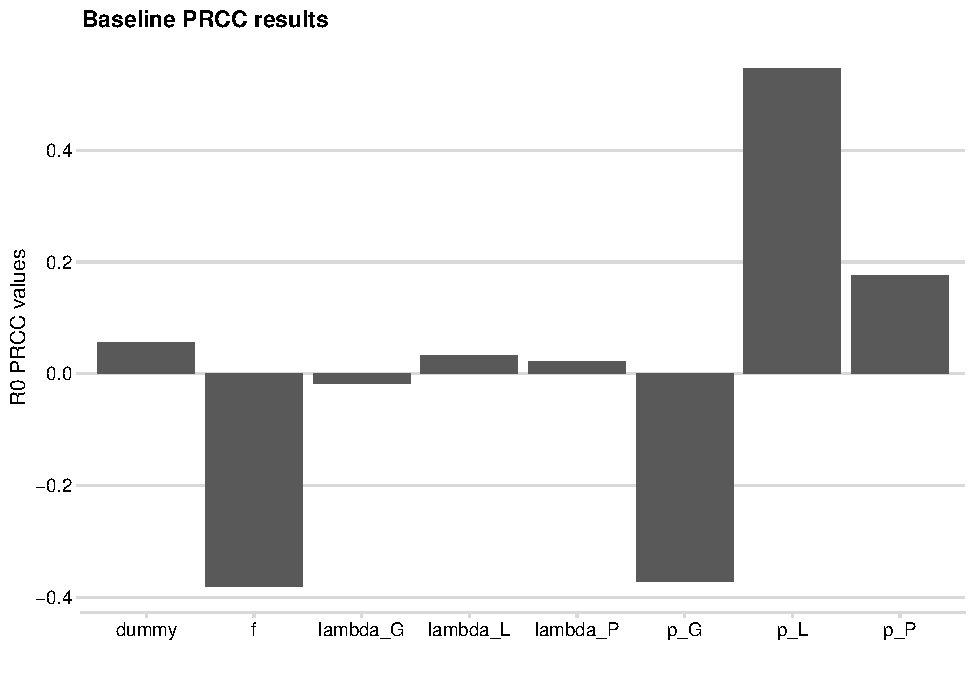
\includegraphics{F:/GitHub/MBF_models/doc/study_files/figure-latex/baseline-prcc-table-1} \caption{Table 3: Baseline PRCC values}\label{fig:baseline-prcc-table}
\end{figure}

\begin{figure}[H]
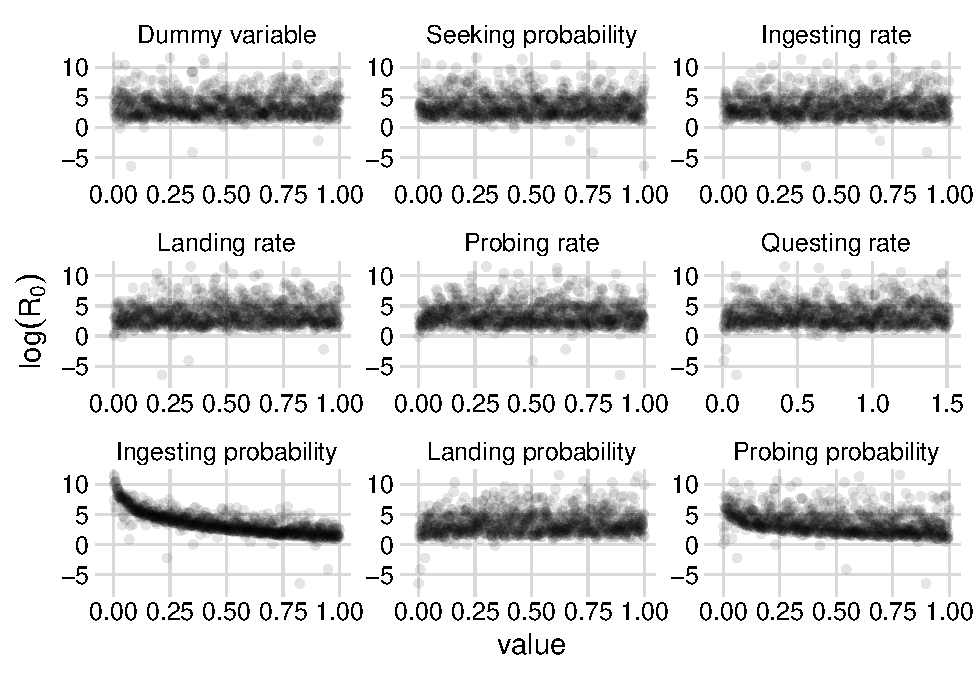
\includegraphics{F:/GitHub/MBF_models/doc/study_files/figure-latex/R0-mono-check-1} \caption{Test for the monotonicity of R0 with respect to Latin hypercube sampled blood-feeding parameters.}\label{fig:R0-mono-check}
\end{figure}

\begin{figure}[H]
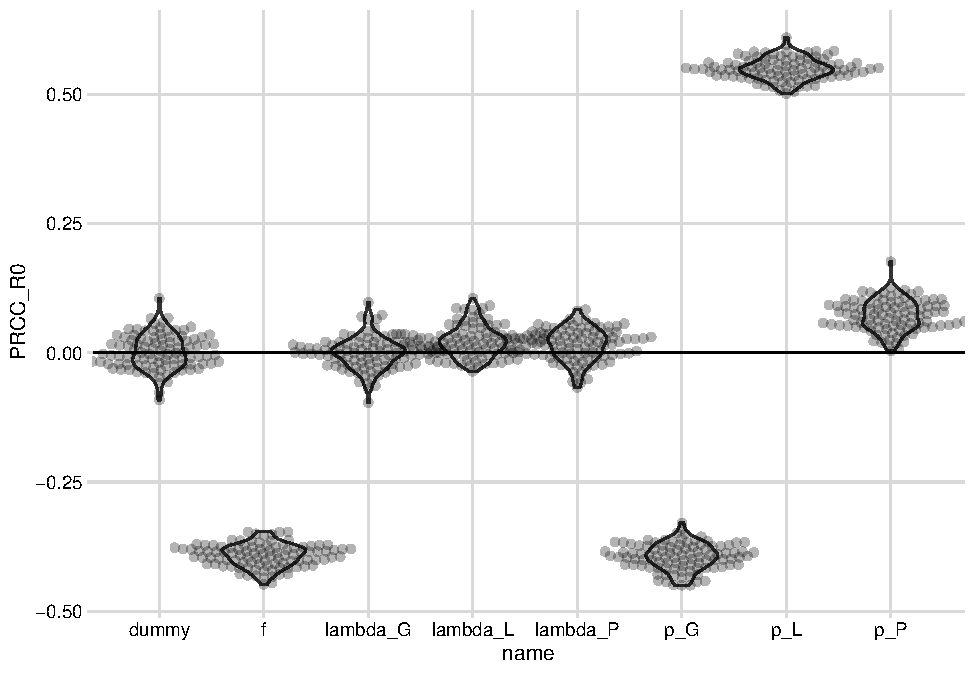
\includegraphics{F:/GitHub/MBF_models/doc/study_files/figure-latex/PRCC_var_test-1} \caption{Diagnostic test of the variation in PRCC values using 10 independent calculations}\label{fig:PRCC_var_test}
\end{figure}

The global sensitivity of \(R_0\) to the biting rate parameters does not
change when the extrinsic incubation period is increased.

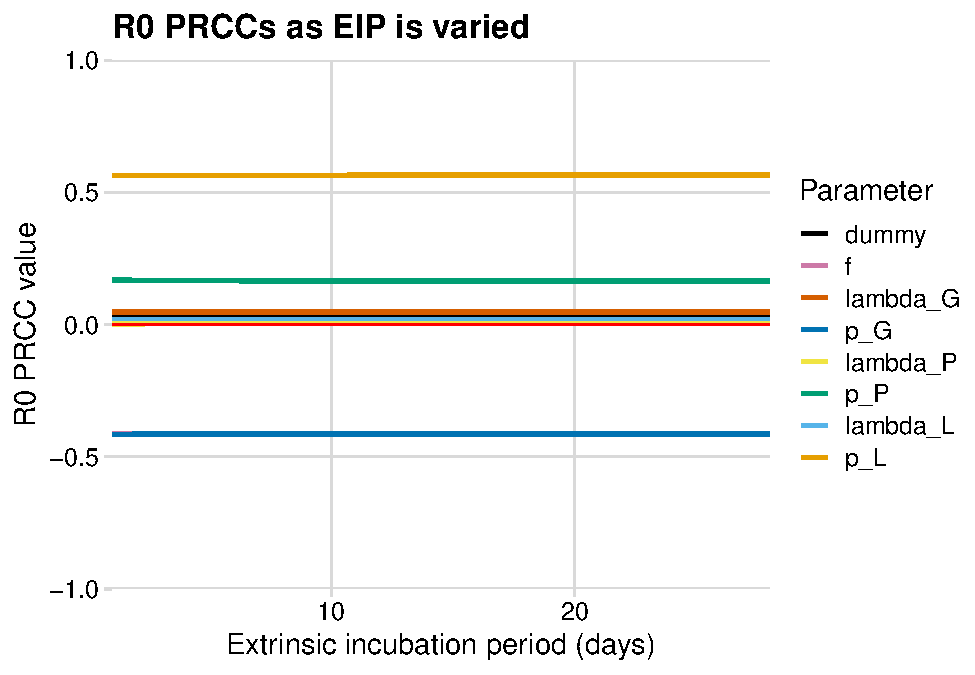
\includegraphics{F:/GitHub/MBF_models/doc/study_files/figure-latex/R0-PRCC-vary-EIP-1}
Similarly, changing the lifespan of the mosquito also does not impact
the global sensitivity of \(R_0\) to the biting rate parameters.

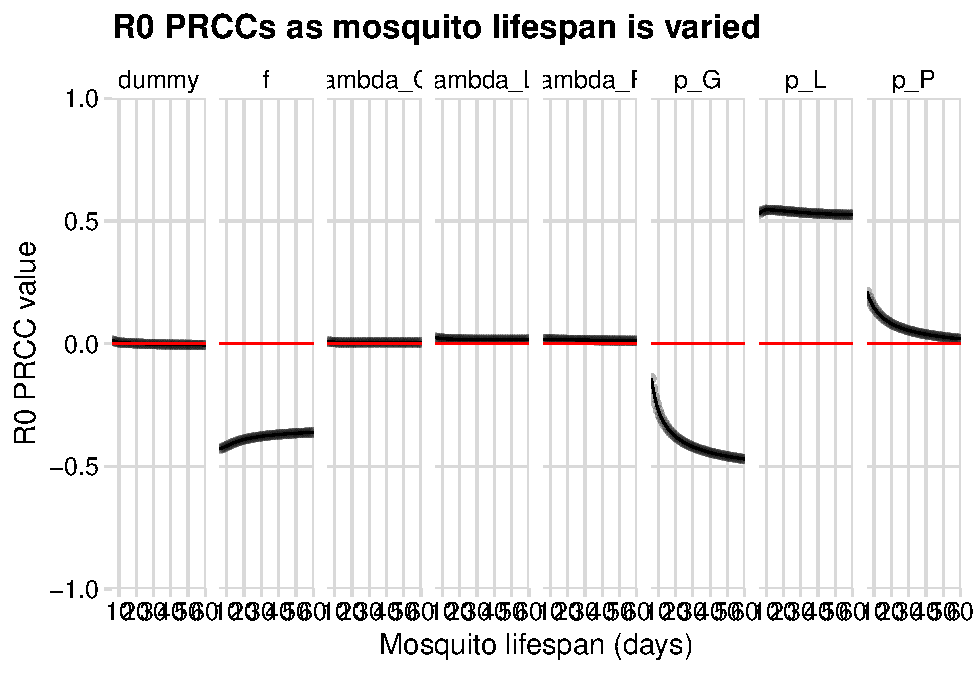
\includegraphics{F:/GitHub/MBF_models/doc/study_files/figure-latex/R0-PRCC-vary-mu-1}
Let's see what happens when we increase the questing time

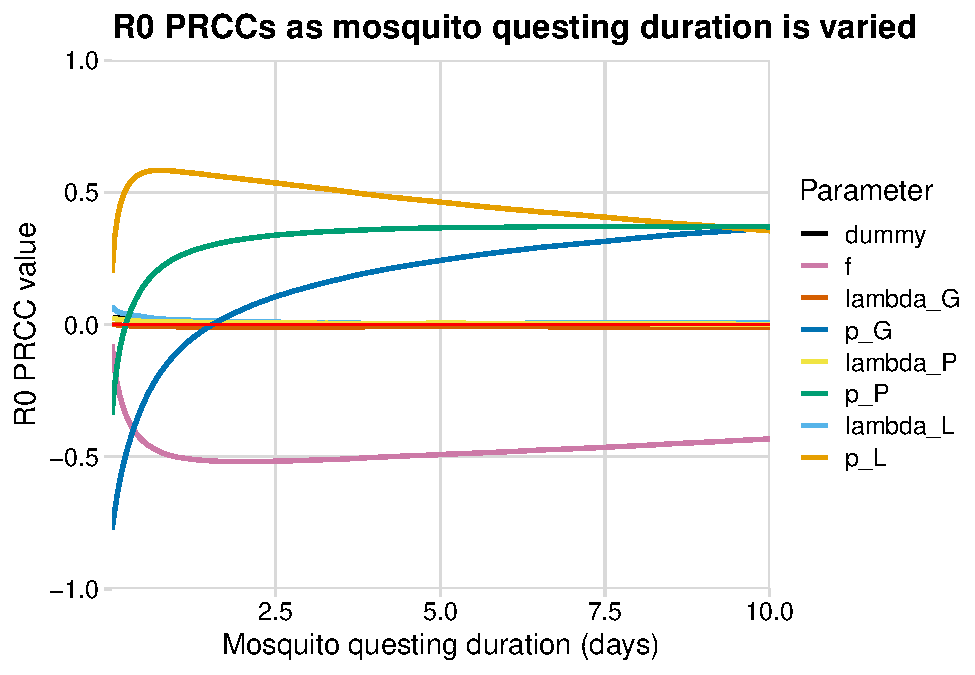
\includegraphics{F:/GitHub/MBF_models/doc/study_files/figure-latex/R0-PRCC-vary-lambdaQ-1}

\section{Results: Uncertainty
analysis}\label{results-uncertainty-analysis}

\subsection{Fitting phase-type
distributions}\label{fitting-phase-type-distributions}

We first need to estimate the parameters of the model from the available
data. Because we are not certain of appropriate way to model the
processes of multiple blood-feeding, we consider three types of models:
empirical, phenomenological, and mechanistic. For the empirical model,
we don't assume to know the actual underlying processes, essentially
considering them a black box. We will consider three orders for this
model: 1 (corresponding to an exponential distribution), 3 (for
comparison with the mechanistic model), and 5. The phenomenological
model focuses are getting the phenomenon right: that there is some
disruption causing mosquitoes to take multiple blood meals. For now, we
consider model orders of 3, 4, and 5. Finally, the mechanistic model
incorporates what we know about the elements of the mosquito
blood-feeding processes to directly estimate the parameters. These
parameters align in definition with those used to simulate the test
data.

For each model class, we use an expectation-maximization algorithm that
uses Markov-chain Monte Carlo sampling to perform Bayesian inference on
the parameter values. This means that we obtain posterior distributions
for each of the parameters (or equivalently the matrix elements of
\(A\)).

\subsubsection{Empirical model}\label{empirical-model}

We can compare the waiting time distributions derived from these models
with our simulated data.

\subsubsection{Mechanistic model}\label{mechanistic-model}

Now considering the mechanistic model. We will make direct comparisons
between this model, the simulated data, and the empirical model. First,
we look at how the waiting time statistics compare.

\begin{figure}[H]
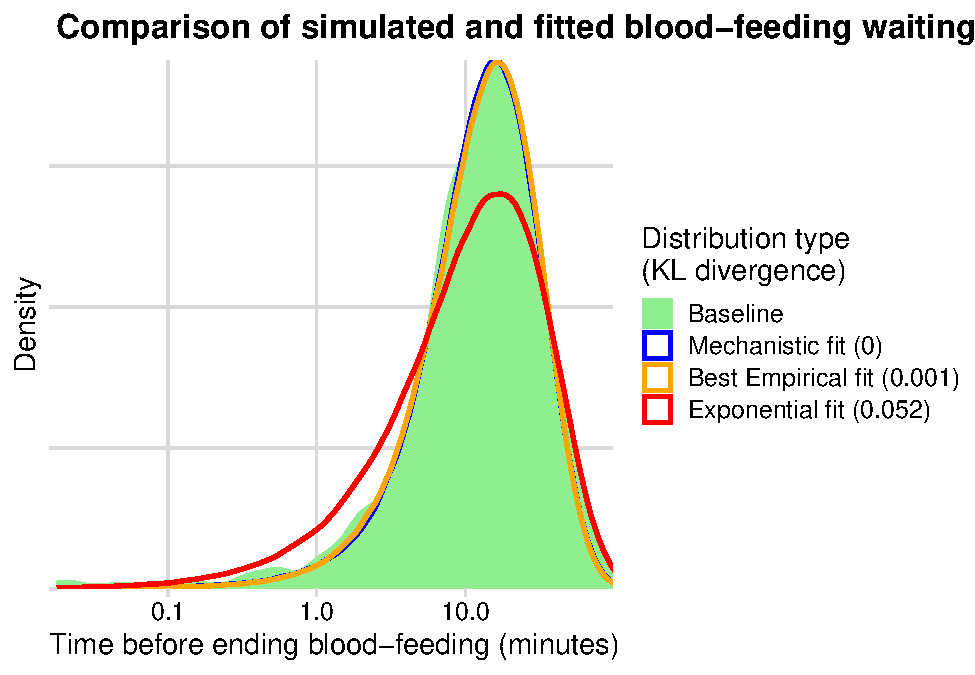
\includegraphics{F:/GitHub/MBF_models/doc/study_files/figure-latex/compare-dists-1} \caption{Comparison of approximated waiting-times for the original simulated data and fitted exponential, empirical phase-type, and mechanistic phase-type distributions.}\label{fig:compare-dists}
\end{figure}

Distributions of the mechanistic parameters compared to the those used
in the simulations.

\begin{verbatim}
## `stat_bin()` using `bins = 30`. Pick better value with `binwidth`.
## `stat_bin()` using `bins = 30`. Pick better value with `binwidth`.
## `stat_bin()` using `bins = 30`. Pick better value with `binwidth`.
\end{verbatim}

\begin{figure}[H]
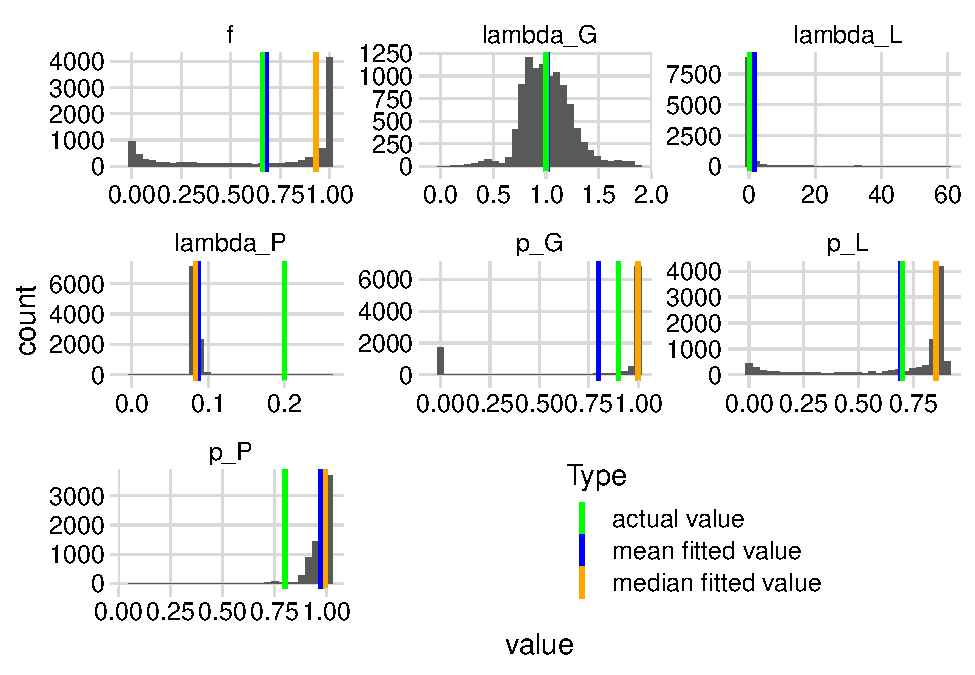
\includegraphics{F:/GitHub/MBF_models/doc/study_files/figure-latex/mech-params-dists-plot-1} \end{figure}

Correlations among the fitted parameters of the mechanistic model

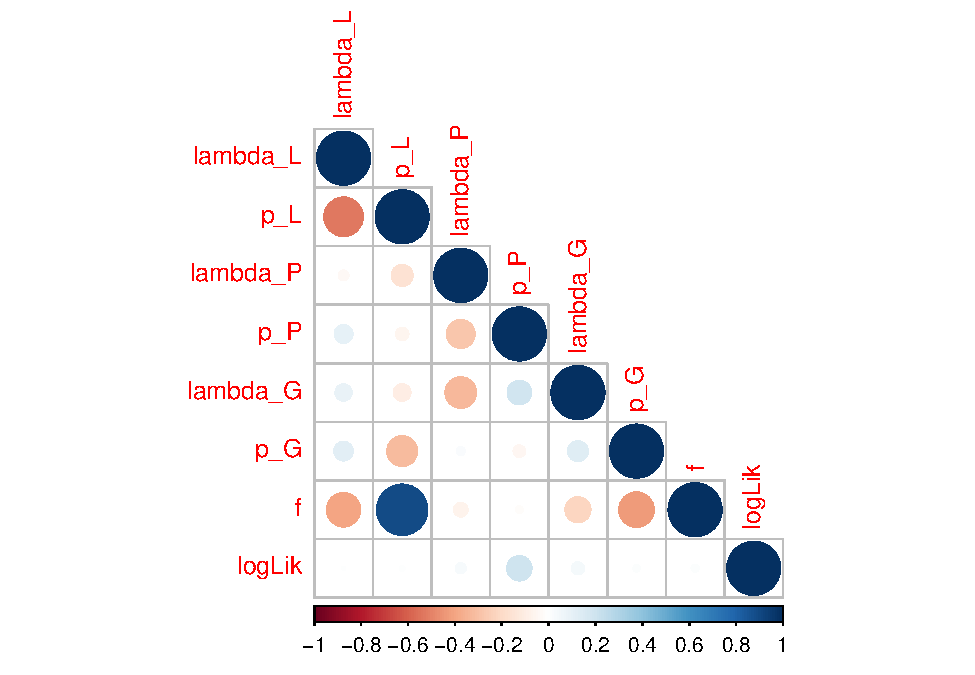
\includegraphics{F:/GitHub/MBF_models/doc/study_files/figure-latex/mech-params-corr-plot-1}

Scatter plots showing associations among mechanistic parameters

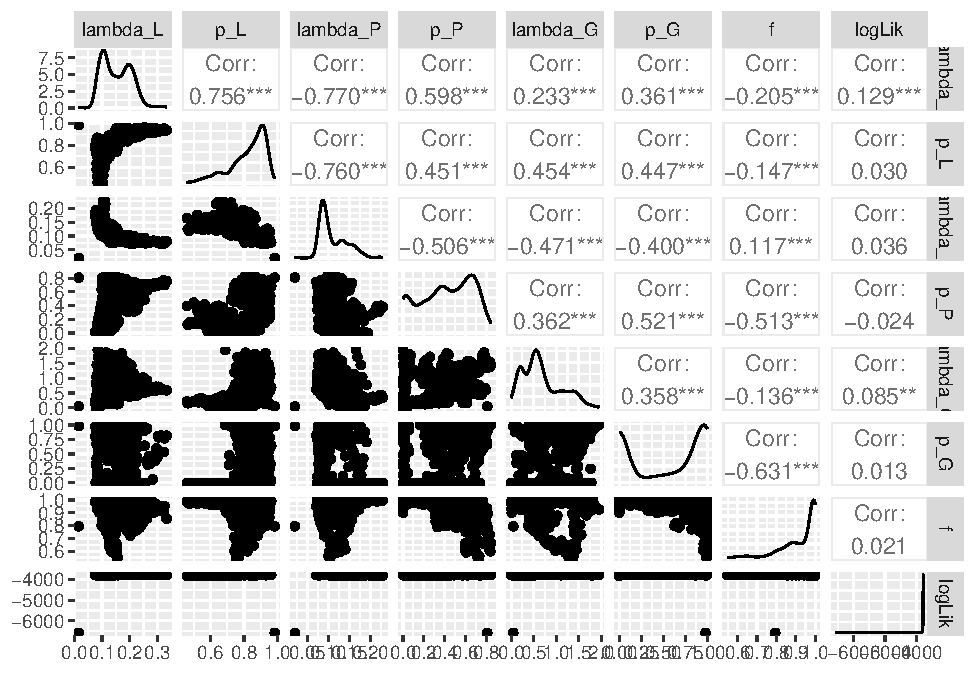
\includegraphics{F:/GitHub/MBF_models/doc/study_files/figure-latex/mech-params-scatter-plot-1}

\subsubsection{Estimates of R0 from fitted parameter
sets}\label{estimates-of-r0-from-fitted-parameter-sets}

Here we study how the blood-feeding parameters affect transmission via
the basic reproduction number.

\section{Discussion}\label{discussion}

\end{document}
